% Document/LinearAlgebra/VectorSpaces/Foundations/DirectSums.tex
% Section: Internal Direct Sums

\newpage
\section{Internal Direct Sums}

\begin{remark}[Motivation]
    A sum $U_1 + U_2 + \cdots + U_k$ of subspaces always produces a subspace, but the
    decomposition of a vector $v = u_1 + u_2 + \cdots + u_k$ may not be unique: different
    choices of $u_i \in U_i$ can give the same $v$. When the decomposition \emph{is} unique
    for every vector in the sum, we have a \textbf{direct sum} --- the strongest and most
    useful way subspaces can combine.

    Direct sums are the subspace-level analogue of linear independence: linear independence
    says each \emph{vector} in a set contributes a genuinely new direction; a direct sum says
    each \emph{subspace} in a family contributes a genuinely new piece of the space. The two
    notions are formally connected by Proposition~\ref{prop:lin-indep-direct-sum}: a set of
    vectors is linearly independent if and only if the one-dimensional subspaces they span
    form a direct sum family.

    In practice, direct sum decompositions appear whenever we decompose a space into
    independent components --- coordinate axes, eigenspaces, invariant subspaces --- and
    the uniqueness of the decomposition is what makes computations in the components
    unambiguous.
\end{remark}

\begin{remark}[Duality with Linear Independence]
    The characterizations of internal direct sums are \textbf{similar} to those of linear independence:
    \begin{itemize}
        \item \textbf{Linear independence}: unique representation of vectors as linear combinations
              of \textbf{vectors} in $L$
        \item \textbf{Direct sum}: unique representation of vectors as sums of \textbf{subspace elements}
              from $(U_i)_{i \in I}$
    \end{itemize}
\end{remark}

\begin{definition}[Unique Representation in a Family of Subspaces]\label{def:unique-rep-subspaces}
    Given a family $(U_i)_{i \in I}$ of subspaces of $V$, a vector $v$ has \textbf{unique representation}
    in the family if there exists a \textbf{unique} finite subset $F \subseteq I$ and \textbf{unique nonzero}
    vectors $(u_i)_{i \in F}$ with $u_i \in U_i$ such that
    \[
        v = \sum_{i \in F} u_i
    \]
    The requirement that components be nonzero ensures uniqueness: otherwise we could add $0 \in U_j$ for any $j$.
\end{definition}

\begin{theorem}[Characterizations of Internal Direct Sums]\label{thm:direct-sum-equiv}
    Let $(U_i)_{i \in I}$ be a family of subspaces of $V$. The following are equivalent:
    \begin{enumerate}
        \item[(i)] $\Forall :{j \in I}{U_j \Intersect \SubspaceSum{i \in I,\, i \neq j}{U_i} = \{0\}}$
        \item[(ii)] Every $v \in \SubspaceSum{i \in I}{U_i}$ has unique representation in the family
        \item[(iii)] Some $v \in \SubspaceSum{i \in I}{U_i}$ with $v \neq 0$ has unique representation
        \item[(iv)] $0$ has unique representation (i.e., if $0 = \sum_{i \in F} u_i$ with $u_i \in U_i$
              nonzero, then $F = \emptyset$)
    \end{enumerate}
\end{theorem}

\begin{proof}
    \textbf{(ii) $\Rightarrow$ (iii)}:
    Trivial (take any nonzero $v$; note $v = 0$ always has unique representation with $F = \emptyset$).

    \textbf{(iii) $\Rightarrow$ (iv)}:
    Let $v \neq 0$ have unique representation $v = \sum_{i \in F} u_i$ with $u_i \neq 0$.
    If $0 = \sum_{j \in G} w_j$ with $w_j \neq 0$, then
    \[
        v = v + 0 = \sum_{i \in F} u_i + \sum_{j \in G} w_j
    \]
    For uniqueness, we need $G = \emptyset$.

    \textbf{(iv) $\Rightarrow$ (ii)}:
    Suppose $v = \sum_{i \in F} u_i = \sum_{j \in G} w_j$ with $u_i, w_j \neq 0$.
    Then $0 = \sum_{i \in F} u_i - \sum_{j \in G} w_j$.
    For $k \in F \Intersect G$: the coefficient is $u_k - w_k \in U_k$.
    For $k \in F \setminus G$: the coefficient is $u_k \in U_k$.
    For $k \in G \setminus F$: the coefficient is $-w_k \in U_k$.
    By (iv), all these must be zero, so $F = G$ and $u_i = w_i$.

    \textbf{(i) $\Rightarrow$ (iv)} (requires field axioms for extraction):
    Suppose $0 = \sum_{i \in F} u_i$ with $u_j \neq 0$ for some $j \in F$.
    Then $u_j = -\sum_{i \in F,\, i \neq j} u_i \in \SubspaceSum{i \in I,\, i \neq j}{U_i}$.
    Also $u_j \in U_j$, so $u_j \in U_j \Intersect \SubspaceSum{i \in I,\, i \neq j}{U_i} = \{0\}$ by (i).
    This contradicts $u_j \neq 0$.

    \textbf{(iv) $\Rightarrow$ (i)}:
    Suppose $u \in U_j \Intersect \SubspaceSum{i \in I,\, i \neq j}{U_i}$ with $u \neq 0$.
    Then $u = \sum_{i \neq j} u_i$ for some $u_i \in U_i$.
    Rearranging: $0 = (-u) + \sum_{i \neq j} u_i$ where $-u \in U_j$.
    The component in $U_j$ is $-u \neq 0$, contradicting (iv).
\end{proof}

\begin{definition}[Internal Direct Sum Family]\label{def:direct-sum-family}
    A family $(U_i)_{i \in I}$ of subspaces is an \textbf{internal direct sum family}
    if it satisfies the equivalent conditions of Theorem~\ref{thm:direct-sum-equiv}.
    We write $\DirectSum{i \in I}{U_i}$ for the sum when the family is a direct sum family.
\end{definition}

\begin{proposition}[Two-Subspace Criterion]\label{prop:two-subspace-direct}
    For two subspaces $U, W \Subspace[K] V$:
    \[
        U + W \text{ is a direct sum} \iff U \Intersect W = \{0\}
    \]
    When this holds, we write $U \DirectSum W$ for the direct sum.
\end{proposition}

\begin{proof}
    Taking $I = \{0, 1\}$ with $U_0 = U$, $U_1 = W$, condition (i) becomes:
    \begin{itemize}
        \item $U \Intersect W = \{0\}$
        \item $W \Intersect U = \{0\}$
    \end{itemize}
    These are equivalent, giving the criterion.
\end{proof}

\begin{example}[Direct Sum Decompositions]\label{ex:direct-sums}
    Consider the following direct sum decompositions:
    \begin{enumerate}
        \item $\bb{R}^3 = $ (xy-plane) $\DirectSum$ (z-axis)
        \item $K^n = \DirectSum{i \in n}{K \cdot \CanonicalVector{i}}$ (direct sum of coordinate axes)
        \item $K[X] = K[X]_{\text{even}} \DirectSum K[X]_{\text{odd}}$ (even/odd degree polynomials)
    \end{enumerate}

    \begin{center}
    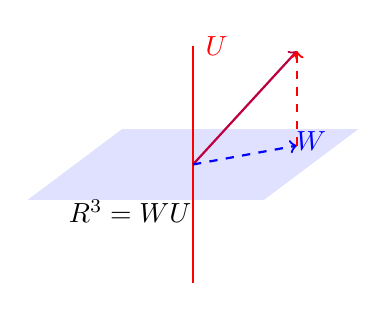
\begin{tikzpicture}[scale=1.0,
        x={(1cm,0cm)},
        y={(0.4cm,0.3cm)},
        z={(0cm,1cm)}]

        % xy-plane
        \fill[blue!20, opacity=0.6] (-1.5,-1.5,0) -- (1.5,-1.5,0) -- (1.5,1.5,0) -- (-1.5,1.5,0) -- cycle;
        \node[blue] at (1.5, 0, 0.3) {$W$};

        % z-axis
        \draw[thick, red] (0,0,-1.5) -- (0,0,1.5);
        \node[red] at (0.3,0,1.5) {$U$};

        % A vector decomposed
        \draw[->, thick, purple] (0,0,0) -- (1,0.8,1.2);
        \draw[->, thick, blue, dashed] (0,0,0) -- (1,0.8,0);
        \draw[->, thick, red, dashed] (1,0.8,0) -- (1,0.8,1.2);

        % Labels
        \node at (0,-2,0) {$\bb{R}^3 = W \DirectSum U$};
    \end{tikzpicture}
    \end{center}
\end{example}

\begin{example}[Non-Direct Sum]\label{ex:non-direct-sum}
    Two distinct lines through the origin in $\bb{R}^3$ do NOT decompose $\bb{R}^3$:
    their sum is only a plane, not all of $\bb{R}^3$.

    However, two distinct lines through the origin in $\bb{R}^2$ DO form a direct sum
    decomposition of $\bb{R}^2$ (assuming they are not the same line).
\end{example}

\begin{proposition}[Linear Independence and Direct Sum]\label{prop:lin-indep-direct-sum}
    Let $F \subseteq V$ and let $(A_i)_{i \in I}$ be a partition of $F$ into linearly
    independent subsets. Then the following are equivalent:
    \begin{enumerate}
        \item $F$ is linearly independent
        \item $(\Span[K]{A_i})_{i \in I}$ is a direct sum family
    \end{enumerate}
\end{proposition}

\begin{proof}
    \textbf{(1) $\Rightarrow$ (2)}:
    Suppose $F$ is linearly independent. We show $(\Span[K]{A_i})_{i \in I}$ satisfies the
    direct sum property (iv): if $0 = \sum_{i \in G} u_i$ with $u_i \in \Span[K]{A_i}$ nonzero,
    then $G = \emptyset$.

    Each $u_i \in \Span[K]{A_i}$ can be written as $u_i = \sum_{v \in B_i} a_{i,v} v$ for some
    finite $B_i \subseteq A_i$ with $a_{i,v} \neq 0$. Thus:
    \[
        0 = \sum_{i \in G} \sum_{v \in B_i} a_{i,v} v
    \]
    Since $(A_i)$ partitions $F$, all these $v$ are distinct elements of $F$.
    By linear independence of $F$ (Theorem~\ref{thm:lin-indep-equiv}(iv)), all $a_{i,v} = 0$.
    But we assumed $a_{i,v} \neq 0$, so each $B_i = \emptyset$, hence each $u_i = 0$.
    This contradicts $u_i \neq 0$, so $G = \emptyset$.

    \textbf{(2) $\Rightarrow$ (1)}:
    Suppose $(\Span[K]{A_i})_{i \in I}$ is a direct sum family. To prove $F$ is linearly
    independent, consider any relation $0 = \sum_{v \in G} a_v v$ with $G \subseteq F$ finite
    and scalars $a_v \in K$; we show that every $a_v = 0$.

    Group the terms by the block of the partition to which each vector belongs: for each
    $i \in I$ put $G_i = G \Intersect A_i$ and
    \[
        u_i = \sum_{v \in G_i} a_v v \in \Span[K]{A_i}.
    \]
    Since $(A_i)$ partitions $F$, the sets $G_i$ are pairwise disjoint with union $G$, so
    \[
        \sum_{i \in I} u_i = \sum_{v \in G} a_v v = 0
    \]
    (a finite sum, as only finitely many $G_i$ are nonempty). By the defining property of a
    direct sum family (characterization (iv)), each $u_i = 0$.

    Now fix $i \in I$. Then $\sum_{v \in G_i} a_v v = u_i = 0$ is a finite linear combination
    of the block $A_i$, which is linearly independent \emph{by hypothesis}; hence $a_v = 0$ for
    every $v \in G_i$. As this holds for all $i$ and the $G_i$ cover $G$, we conclude $a_v = 0$
    for every $v \in G$. Therefore $F$ is linearly independent.
\end{proof}

\begin{corollary}[Singleton Partition Case]\label{cor:lin-indep-singleton-partition}
    Let $F \subseteq V$ with $0 \notin F$. Then $F$ is linearly independent if and only if
    $(\Span[K]{\{v\}})_{v \in F}$ is a direct sum family with sum $\Span[K]{F}$.
\end{corollary}

\begin{proof}
    Since $0 \notin F$, each singleton block $\{v\}$ (for $v \in F$) is linearly independent;
    hence $(\{v\})_{v \in F}$ is a partition of $F$ into linearly independent subsets, and
    Proposition~\ref{prop:lin-indep-direct-sum} applies to give the stated equivalence. The
    hypothesis $0 \notin F$ cannot be dropped: a block $\Span[K]{\{0\}} = \{0\}$ satisfies the
    direct-sum condition vacuously, so for $F \ni 0$ the family would be a direct sum family
    even though $F$ is linearly dependent. Finally, the sum of the family is
    \[
        \SubspaceSum{v \in F}{\Span[K]{\{v\}}}
        = \Span[K]{\BigUnion[v \in F] \{v\}}
        = \Span[K]{F}
    \]
    (sum of spans equals the span of the union), independently of directness.
\end{proof}

\begin{proposition}[Direct Sum Characterization via Linear Independence]\label{prop:direct-sum-lin-indep}
    A family $(U_i)_{i \in I}$ is a direct sum family if and only if for any linearly independent
    sets $F_i \subseteq U_i$, the union $\BigUnion[i \in I] F_i$ is linearly independent.
\end{proposition}

\begin{proof}
    ($\Rightarrow$)
    Suppose $(U_i)$ is a direct sum family. Let $F_i \subseteq U_i$ be linearly independent for each $i$.
    Suppose $0 = \sum_{k} a_k v_k$ where $v_k \in \BigUnion[i \in I] F_i$ with $a_k \neq 0$.
    Group by index: $0 = \sum_{i} (\sum_{v \in F_i} a_v v)$.
    Each inner sum $u_i = \sum_{v \in F_i} a_v v \in \Span[K]{F_i} \subseteq U_i$.
    By the direct sum property, each $u_i = 0$.
    By linear independence of $F_i$, all $a_v = 0$, so the only representation of $0$ is the empty sum.
    Hence $\BigUnion[i \in I] F_i$ is linearly independent.

    ($\Leftarrow$)
    We prove $(U_i)$ satisfies the direct sum property (iv): if $0 = \sum_{i \in G} u_i$ with
    $u_i \in U_i$ nonzero, then $G = \emptyset$.

    Suppose $0 = \sum_{i \in G} u_i$ with $u_i \neq 0$ for all $i \in G$.
    For each $i \in G$, the singleton $\{u_i\} \subseteq U_i$ is linearly independent (since $u_i \neq 0$).
    By assumption, $\BigUnion[i \in G] \{u_i\}$ is linearly independent.
    But $0 = \sum_{i \in G} 1 \cdot u_i$ is a nontrivial representation of zero,
    contradicting linear independence. Hence $G = \emptyset$.
\end{proof}

\begin{definition}[Direct Sum Decomposition of $V$]\label{def:direct-decomposition}
    We say $V$ \textbf{decomposes} as a direct sum $V = \DirectSum{i \in I}{U_i}$ if:
    \begin{enumerate}
        \item $(U_i)_{i \in I}$ is a direct sum family
        \item $V = \SubspaceSum{i \in I}{U_i}$
    \end{enumerate}
    Equivalently: every $v \in V$ has unique representation in the family.
\end{definition}
